\documentclass[aspectratio=169]{beamer}

%\usepackage[table]{xcolor}
\mode<presentation> {
  \usetheme{Boadilla}
%  \usetheme{Pittsburgh}
%\usefonttheme[2]{sans}
\renewcommand{\familydefault}{cmss}
%\usepackage{lmodern}
%\usepackage[T1]{fontenc}
%\usepackage{palatino}
%\usepackage{cmbright}
  %\setbeamercovered{transparent}
\useinnertheme{rectangles}
}
%\usepackage{normalem}{ulem}
%\usepackage{colortbl, textcomp}
\setbeamercolor{normal text}{fg = black}
\setbeamercolor{structure}{fg = blue}
\definecolor{trial}{cmyk}{1,0,0, 0}
\definecolor{trial2}{cmyk}{0.00,0,1, 0}
\definecolor{darkgreen}{rgb}{0,.4, 0.1}
\definecolor{mygray}{gray}{0.8}
\definecolor{myblack}{rgb}{0, 0, 0}
\usepackage{array}
\beamertemplatesolidbackgroundcolor{white}  \setbeamercolor{alerted
text}{fg=red}

\setbeamertemplate{caption}[numbered]\newcounter{mylastframe}

\usepackage{color}
\usepackage{tikz}
\usetikzlibrary{arrows}
\usepackage{colortbl}
\usepackage{graphicx}
\usepackage{epsfig}

%\usepackage[usenames, dvipsnames]{color}
%\setbeamertemplate{caption}[numbered]\newcounter{mylastframe}c
%\newcolumntype{Y}{\columncolor[cmyk]{0, 0, 1, 0}\raggedright}
%\newcolumntype{C}{\columncolor[cmyk]{1, 0, 0, 0}\raggedright}
%\newcolumntype{G}{\columncolor[rgb]{0, 1, 0}\raggedright}
%\newcolumntype{R}{\columncolor[rgb]{1, 0, 0}\raggedright}

%\begin{beamerboxesrounded}[upper=uppercol,lower=lowercol,shadow=true]{Block}
%$A = B$.
%\end{beamerboxesrounded}}
\renewcommand{\familydefault}{cmss}
%\usepackage[all]{xy}

\usepackage{tikz}
\usepackage{lipsum}

 \newenvironment{changemargin}[3]{%
 \begin{list}{}{%
 \setlength{\topsep}{0pt}%
 \setlength{\leftmargin}{#1}%
 \setlength{\rightmargin}{#2}%
 \setlength{\topmargin}{#3}%
 \setlength{\listparindent}{\parindent}%
 \setlength{\itemindent}{\parindent}%
 \setlength{\parsep}{\parskip}%
 }%
\item[]}{\end{list}}
\usetikzlibrary{arrows}
%\usepackage{palatino}
%\usepackage{eulervm}
\usecolortheme{lily}

\newtheorem{com}{Comment}
\newtheorem{lem} {Lemma}
\newtheorem{prop}{Proposition}
\newtheorem{thm}{Theorem}
\newtheorem{defn}{Definition}
\newtheorem{cor}{Corollary}
\newtheorem{obs}{Observation}
 \numberwithin{equation}{section}


\title[PLSC 43401] % (optional, nur bei langen Titeln ng)
{Mathematical Foundations of Political Methodology Lecture 2}

\author{Robert Gulotty}
\institute[University of Chicago]{Department of Political Science \\  University of Chicago}
\vspace{0.3in}
\date{August 28th, 2017}

\setbeamertemplate{navigation symbols}{}

\begin{document}

\begin{frame}
\titlepage
\end{frame}


\begin{frame}{Recap/motivation}

Claim:  The empty set $\emptyset$ is a subset of every set. \pause

 \begin{center}
 \underline{Direct proof}:\\\pause
 \end{center}
Recall ``subset'',  $B\subset A$, is \emph{defined} to mean:\\
  
 \begin{center}
\fbox{\begin{minipage}{15em}

 ``For all x in the set B, those x are also in the set A.''\\
$$\forall x\in B,\quad   x\in A$$ 
\end{minipage}
}
\end{center}
\pause

``The empty set $\emptyset$ is a subset of every set.'' can be rewritten, 
$$\forall A,\ \forall x\in \emptyset,\ \quad  x\in A$$
\pause 
Pick an arbitrary set A.  We then test whether or not those $x\in \emptyset$ satisfy $x\in A$. But we know that there are no $x\in \emptyset$. \pause
$$\forall x\in \emptyset,\ \quad  x\in A, \quad \Box$$  

\end{frame}


\begin{frame}{Why Proofs?}

\begin{itemize}
\item Proofs are just arguments that use logical reasoning.\pause
\item Logical reasoning is a skill obtainable via practice and study.\pause
\item Formal theory can remove ambiguity and imprecision, creating possibility for surprising discoveries: Arrow Impossibility Theorem.\pause
\item Today we will focus on demystification and vocabulary.
\end{itemize}

\end{frame}





\begin{frame}{Today's plan}

\begin{itemize}
\item \textcolor{myblack}{Logical Notation}
\item \textcolor{myblack}{Methods of Mathematical Proof}
\item \textcolor{myblack}{Social Scientific Thinking}
\end{itemize}

\end{frame}




\begin{frame}
\frametitle{Proposition}

\begin{defn}
A \textbf{proposition} is a statement that is either true or false.
\end{defn} \pause

\ \\Three examples: \pause

\ \\Proposition: $2 + 3 = 5$. \pause

\ \\Proposition: Oranges are a kind of vegetable. \pause

\ \\Proposition: Superstition is the belief in the causal nexus.

\end{frame}



\begin{frame}
\frametitle{Proposition}

\ \\In English, we can modify, combine, and relate propositions with words such as ``not''', ``and", ``implies'', and ``if-then''. Such propositions are called as compound propositions. \pause
\begin{table}[]
\begin{tabular}{lll}
English&In R& Symbols \\
\hline
``not'' &\texttt{!} (Bang) & $\sim$\\
``and'' & \texttt{\&} & $\cap$\\
``or'' & \texttt{|} (Pipe)& $\cup$\\
``if-then'' & \texttt{ifelse}& $\rightarrow$ \\
\end{tabular}
\end{table} \pause
\ \\To understand compound propositions, we can use \emph{truth tables}.

\end{frame}



\begin{frame}
\frametitle{Truth Table}
Truth tables were popularized by Ludwig Wittgenstein in his \emph{Tractatus Logico-Philosophicus}
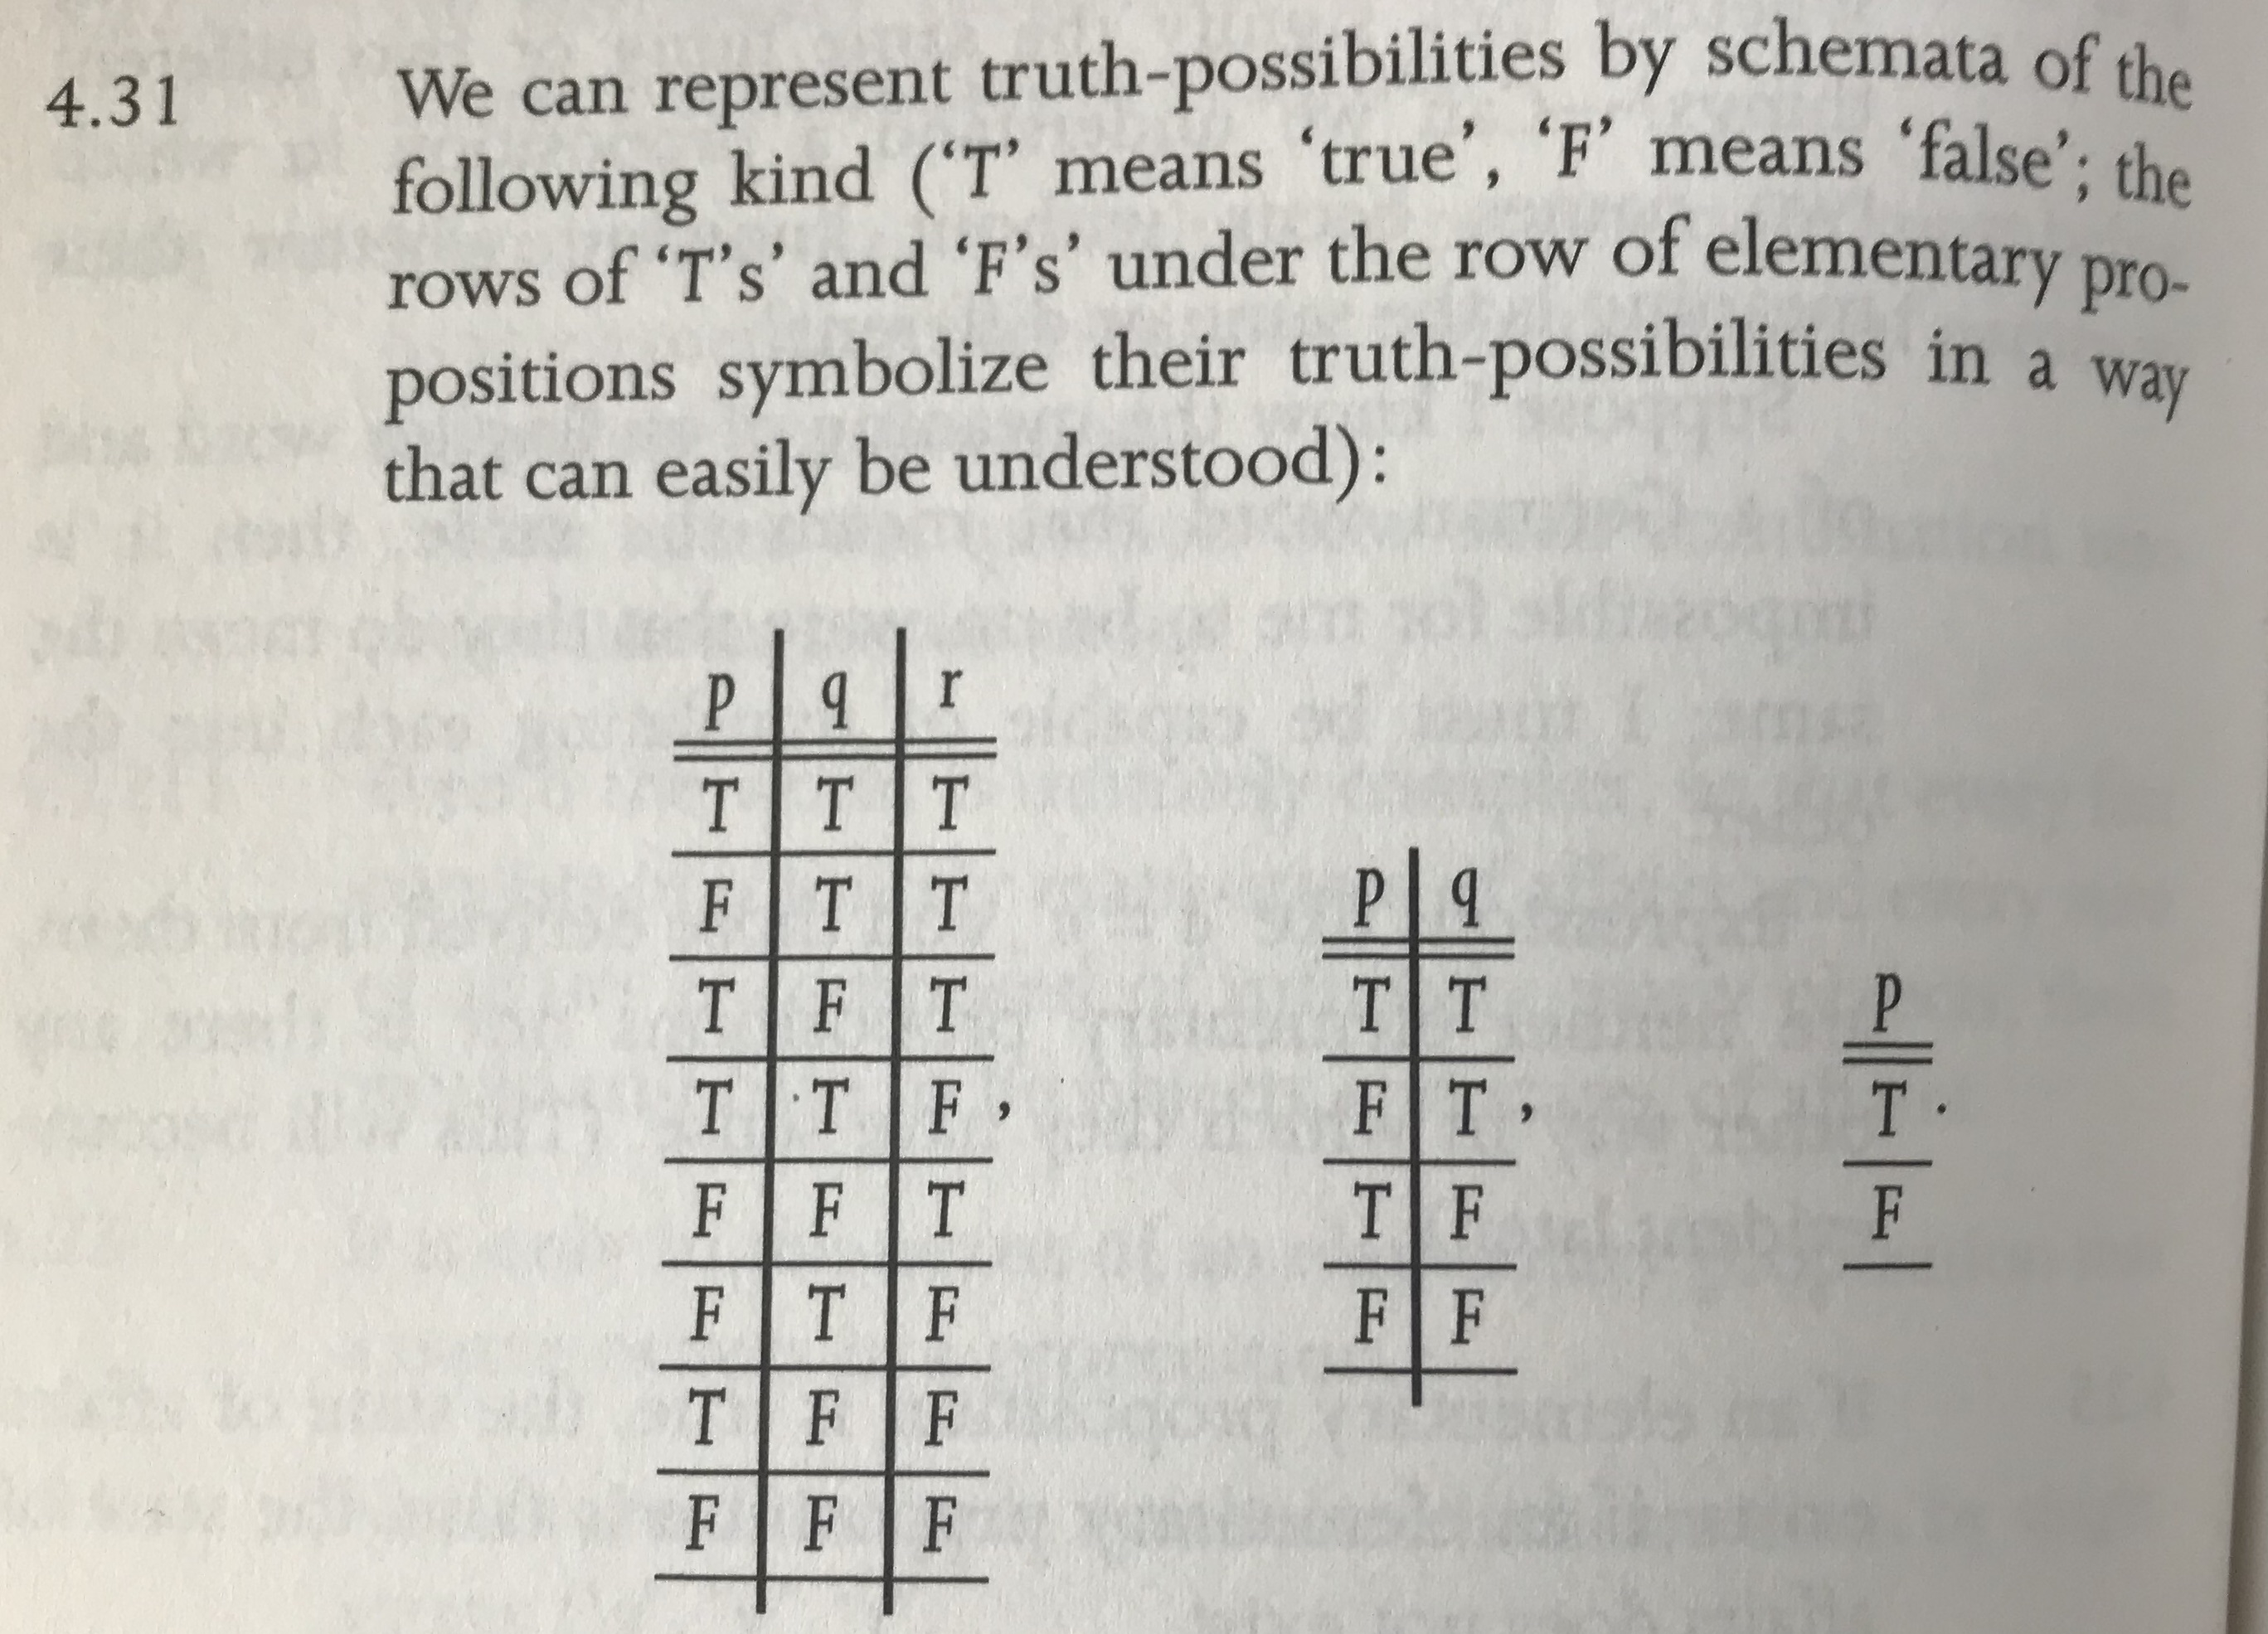
\includegraphics[width=3.5 in]{Tractatus.jpg}


\end{frame}


\begin{frame}
\frametitle{Proposition: Not(P)}

\ \\The truth table for "Not(P)" is:

\begin{table}[]
\begin{tabular}{lllll}
P                     & Not(P)                &  &  &  \\ \cline{1-2}
\multicolumn{1}{c}{T} & \multicolumn{1}{c}{F} &  &  &  \\
\multicolumn{1}{c}{F} & \multicolumn{1}{c}{T} &  &  &  \\
                      &                       &  &  & 
\end{tabular}
\end{table}

\end{frame}



\begin{frame}
\frametitle{Proposition: P and Q}

\ \\The truth table for "P and Q" is:

\begin{table}[]
\begin{tabular}{cccll}
\multicolumn{1}{l}{P} & \multicolumn{1}{l}{Q} & \multicolumn{1}{l}{P and Q} &  &  \\ \cline{1-3}
T                     & T                     & T                           &  &  \\
T                     & F                     & F                           &  &  \\
F                     & T                     & F                           &  &  \\
F                     & F                     & F                           &  & 
\end{tabular}
\end{table} 


\end{frame}



\begin{frame}
\frametitle{Proposition: P or Q}

\ \\The truth table for``P or Q" is:

\begin{table}[]
\begin{tabular}{cccll}
\multicolumn{1}{l}{P} & \multicolumn{1}{l}{Q} & \multicolumn{1}{l}{P or Q} &  &  \\ \cline{1-3}
T                     & T                     & T                          &  &  \\
T                     & F                     & T                          &  &  \\
F                     & T                     & T                          &  &  \\
F                     & F                     & F                          &  & 
\end{tabular}
\end{table}

\end{frame}



\begin{frame}
\frametitle{Proposition: Implication ($P\rightarrow Q$)}

In an `if then' statement, we say the antecedent $P$ implies the consequent $Q$.\\

\ \\The truth table for "P implies Q" is:

\begin{table}[]
\begin{tabular}{cccll}
\multicolumn{1}{l}{P} & \multicolumn{1}{l}{Q} & \multicolumn{1}{l}{P implies Q} &  &  \\ \cline{1-3}
T                     & T                     & T                               &  &  \\
T                     & F                     & F                               &  &  \\
F                     & T                     & T                               &  &  \\
F                     & F                     & T                               &  & 
\end{tabular}
\end{table} \pause

\ \\In words: 
\begin{itemize}
\item An implication is true exactly when the if-part is false or the then-part is true. 
\item In words: An implication is false exactly when the if-part is true and the then-part is false. 
\pause
\item ``If my grandmother had wheels then she would have been a bike.''
\end{itemize}
\end{frame}


\begin{frame}
\frametitle{Alternative Intuition for Implication}

\ \\The truth table for ``not(P) or Q'' is:

\begin{table}[]
\begin{tabular}{ccccl}
\multicolumn{1}{l}{P} & \multicolumn{1}{l}{Q} & \multicolumn{1}{l}{not(P)} & \multicolumn{1}{l}{not(P) V Q}   &  \\ \cline{1-4}
T                     & T                     & F                              &   T          &  \\
T                     & F                     & F                               & F &  \\
F                     & T                     & T                               & T &  \\
F                     & F                     & T                               & T & 
\end{tabular}
\end{table} \pause
Note that this is the same as implication.
\end{frame}


\begin{frame}
\frametitle{Exercise: Pierce Law (1885)}

\ \\ ((P $\rightarrow $ Q)$\rightarrow$ P) $\rightarrow $ P

\begin{table}[]
\begin{tabular}{ccccc}
\multicolumn{1}{l}{P} & \multicolumn{1}{l}{Q} & P$\rightarrow$Q & (P $\rightarrow $Q)$\rightarrow $P & ((P $\rightarrow $ Q)$\rightarrow$ P) $\rightarrow $ P\\ \cline{1-5}
T                     & T                   \\
T                     & F                  \\
F                     & T               \\
F                     & F                
\end{tabular}
\end{table}

\end{frame}




\begin{frame}
\frametitle{Proposition: P IFF Q}

\ \\The truth table for P IFF (if and only if) Q is:

\begin{table}[]
\begin{tabular}{cccll}
\multicolumn{1}{l}{P} & \multicolumn{1}{l}{Q} & \multicolumn{1}{l}{P IFF Q} &  &  \\ \cline{1-3}
T                     & T                     & T                               &  &  \\
T                     & F                     & F                               &  &  \\
F                     & T                     & F                               &  &  \\
F                     & F                     & T                               &  & 
\end{tabular}
\end{table} \pause

\ \\Example. This if-and-only-if statement is true for every real number $x$: $x^{2} - 4 \geq 0$ iff $|x| \geq 2$

\end{frame}



\begin{frame}
\frametitle{Example of IFF ($\iff$)}
\begin{itemize}
\item Prove that: If A, B, and C are sets, then 
$$A \setminus (B \cap C)=(A \setminus B) \cup (A \setminus C).$$\pause
\item[A)] Assume if part (that A, B and C are sets).\pause
\item[B)] Assume left hand side of equation, show right hand side follows $(\subseteq)$.\pause
\item[] Pick any $x\in A \setminus (B \cap C)$.  Then $x\in A$ and $x \notin (B\cap C)$.\pause
\item[] $x \notin (B\cap C)$ means either $x\notin B$ or $x\notin C$.\pause
\item[B.1)] Two Cases\pause
\begin{enumerate}
\item Suppose $x\notin B$. \pause
\item[] We know $x\in A$, so $x\in A \setminus B$. \pause
\item[] If  $x\in A \setminus B$, we know that  $(A \setminus B) \cup (A  \setminus C).$\pause
\item Suppose $x\notin C$. \pause
\item[] We know $x\in A$, so $x\in A \setminus C$. \pause
\item[] If  $x\in A \setminus C$, we know that  $(A \setminus B) \cup (A \setminus C).$\pause
\end{enumerate}
\item[B.2)] So $A \setminus (B \cap C)\subseteq(A \setminus B) \cup (A \setminus C).$
\end{itemize}

\end{frame}

\begin{frame}
\frametitle{Example of IFF ($\iff$)}
\begin{itemize}

\item[C)] Assume right hand side of equation, show left hand side follows $(\supseteq)$.\pause
\item[] Pick any $y\in (A \setminus B) \cup (A \setminus C)$.  Then $y\in A \setminus B$ or $y \in (A\setminus C)$.\pause
\item[C.1)] Two Cases\pause
\begin{enumerate}
\item Suppose $y\in A \setminus B$. \pause
\item[] We know $y\in A$ and $y\notin B$ so $y\notin B\cap C$. \pause
\item[] $y\notin B\cap C$ means $y \in A \setminus (B\cap C)$\pause
\item Suppose $y\in A \setminus C$. \pause
\item[] We know $y\in A$ and $y\notin C$ so $y\notin B\cap C$. \pause
\item[] $y\notin B\cap C$ means $y \in A \setminus (B\cap C)$\pause
\end{enumerate}
\item[C.2)] So $A \setminus (B \cap C)\supseteq(A \setminus B) \cup (A \setminus C).$
\item[D)] So from B.2 and C.2, $A \setminus (B \cap C)=(A \setminus B) \cup (A \setminus C).$
\end{itemize}

\end{frame}






\begin{frame}
\frametitle{Proposition: Contrapositive}

\begin{defn}
``Not(Q) implies Not(P)'' or  $\sim Q \rightarrow \sim P$ is called the \textbf{contrapositive} of the implication ``P implies Q''. \end{defn} \pause

\ \\Their truth table is:

\begin{table}[]
\begin{tabular}{cc|c|cc|c}
\multicolumn{1}{l}{P} & \multicolumn{1}{l}{Q} & \multicolumn{1}{l}{P $\rightarrow$ Q} & $\sim Q$& $\sim P$& $\sim Q \rightarrow \sim P$   \\ \cline{1-6}
T                     & T                     & T       &     F    &     F          & T                       \\
T                     & F                     & F        &     T     &     F        & F                       \\
F                     & T                     & T          &    F       &    T      & T                       \\
F                     & F                     & T           &    T        &    T    & T                     
\end{tabular}
\end{table} \pause

\ \\Example. ``If I am hungry, then I am grumpy.'' is equivalent to ``If I am not grumpy, then I am not hungry''. 

\end{frame}



\begin{frame}
\frametitle{Proposition: Always vs. Sometimes True}

\ \\Examples on "Always True": \pause

\ \\For all $x \in \mathbb{R}$, $x^{2} \geq 0$. Equivalent to write as: $\forall x \in \mathbb{R}$, $x^{2} \geq 0$. \pause

\ \\Examples on "Sometimes True": \pause

\ \\There exists an $x \in \mathbb{R}$ such that $5 x^{2} - 7 = 0$. Equivalent to write as: $\exists x \in \mathbb{R}$ such that $5 x^{2} - 7 = 0$.

\end{frame}




\begin{frame}

\begin{itemize}
\item \textcolor{mygray}{Logical Notation}
\item \textcolor{myblack}{Methods of Mathematical Proof}
\item \textcolor{mygray}{Social Scientific Thinking}
\end{itemize}

\end{frame}



\begin{frame}
\frametitle{Mathematical Proofs}

\ \\Before we proceed to the definition of mathematical proofs, we need to define axioms first. \pause

\begin{defn}
Propositions that are simply accepted as true are called \textbf{axioms}.
\end{defn} \pause

\ \\Example of an axiom: There is a straight line segment between every pair of points.

\end{frame}



\begin{frame}
\frametitle{Mathematical Proofs}

\begin{defn}
A \textbf{mathematical proof} of a proposition is a chain of logical deductions leading to the proposition from a base set of axioms.
\end{defn}

\end{frame}



\begin{frame}
\frametitle{Classes of Results}

The importance of a proposition is indicated with its classification: \pause

\begin{itemize}
\item Very important propositions are called \textbf{theorems}. \pause
\item A \textbf{lemma} is a preliminary proposition useful for proving later propositions. \pause
\item A \textbf{corollary} is a proposition that follows in just a few logical steps from a lemma or a theorem.
\end{itemize}

\end{frame}



\begin{frame}
\frametitle{Methods for Mathematical Proofs}

\ \\A fundamental logical deduction is \emph{modus ponens}.  The truth of P and $P \rightarrow Q$ gives us the truth of Q. \pause

\begin{table}[]
\begin{tabular}{ccl}
\multicolumn{1}{l}{P,} & \multicolumn{1}{l}{P $\rightarrow$ Q} &  \\ \cline{1-2}
\multicolumn{2}{c}{Q}                                    &  \\
\end{tabular}
\end{table} \pause

\ \\An example of an argument that fits the form \emph{modus ponens:} \pause
\ \\If there is a skateboard on the sidewalk, my dog will bark at it.
\ \\There is a skateboard on the sidewalk.\pause
\ \\Therefore, my dog will bark.

\end{frame}

\begin{frame}{Source of \emph{modus ponens}}

\begin{table}[]
\begin{tabular}{cccll}
\multicolumn{1}{l}{P} & \multicolumn{1}{l}{Q} & \multicolumn{1}{l}{P implies Q} &  &  \\ \cline{1-3}
\textbf{T}                     & T                     & \textbf{T}                              &  &  \\
\textbf{T}                     & F                     & F                               &  &  \\
F                     & T                     & \textbf{T}                                &  &  \\
F                     & F                     & \textbf{T}                               &  & 
\end{tabular}
\end{table} 

\end{frame}

\begin{frame}
\frametitle{Classic Logical Fallacy}

\ \\The following error in logic is called `affirming the consequent':\pause
\ \\I assume ``If there is a skateboard on the sidewalk, my dog will bark at it.''
\ \\and see ``My dog is barking.''\pause
\ \\and erroneously conclude:``Therefore, there is a skateboard on the sidewalk.''\pause

\begin{table}
\begin{tabular}{ccl}
\multicolumn{1}{l}{Q,} & \multicolumn{1}{l}{P $\rightarrow$ Q} &  \\ \cline{1-2}
\multicolumn{2}{c}{$P\ \lor \sim P$}                                    &  \\
\end{tabular}
\end{table} 
\end{frame}

\begin{frame}{Source of affirming the consequent}

\begin{table}
\begin{tabular}{cccll}
\multicolumn{1}{l}{P} & \multicolumn{1}{l}{Q} & \multicolumn{1}{l}{P implies Q} &  &  \\ \cline{1-3}
T                  & \textbf{T}                      & \textbf{T}                              &  &  \\
T                   & F                     & F                               &  &  \\
F                     & \textbf{T}                      & \textbf{T}                                &  &  \\
F                     & F                     & \textbf{T}                               &  & 
\end{tabular}
\end{table} 
\end{frame}


\begin{frame}
\frametitle{Methods for Mathematical Proofs: Direct Proof}

\ \\So far we have shown that if we believe $P \rightarrow Q$, and $P$, $Q$ follows.

Most political science claims are like $P \rightarrow Q$, so how do we prove this?  \\

The most common form of proof is the \emph{Direct Proof} \pause

\ \\For this method, in order to prove that $P \rightarrow Q$, there are two steps: 1. Assume P is true; 2. Show that Q logically follows, usually from the definition of P. 

\end{frame}

\begin{frame}{Source of \emph{Direct Proofs}}

\begin{table}[]
\begin{tabular}{cccll}
\multicolumn{1}{l}{P} & \multicolumn{1}{l}{Q} & \multicolumn{1}{l}{P implies Q} &  &  \\ \cline{1-3}
\textbf{T}                     & \textbf{T}                      &T                             &  &  \\
\textbf{T}                     & F                     & F                               &  &  \\
F                     & T                     & T                             &  &  \\
F                     & F                     & T                             &  & 
\end{tabular}
\end{table} 
\end{frame}


\begin{frame}
\frametitle{Methods of Mathematical Proof: Direct Proof}

\begin{theorem}
If $0 \leq x \leq 2$, then, $- x^{3} + 4x + 1 > 0$.
\end{theorem} \pause

\begin{proof}
Assume $0 \leq x \leq 2$. \pause
Then, $x$, $2 - x$, and $2 + x$ are all nonnegative. \pause
Therefore, the product of these terms is also nonnegative. Adding 1 to this product gives a positive number, so:
$$x (2 - x) (2 + x) + 1 \geq 0$$ \pause
Which is equivalent to:
$$- x^{3} + 4x + 1 > 0$$
\end{proof}

\end{frame}



\begin{frame}
\frametitle{Methods of Mathematical Proof: Direct Proof}

Now, let's see an example of using direct proof in set theory. \pause

\begin{thm} Let $A$ and $B$ be sets.  If $A$ = $B$ then $A \subset B$ and $B \subset A$ 
\end{thm}
\pause
\invisible<1>{ \begin{proof}  Suppose $A = B$.  \pause By definition, if $x \in A$ then $x \in B$.  So $A \subset B$.  \pause Again, by definition, if $y \in B$ then $y \in A$.  So $B \subset A$. \end{proof}}

\end{frame}



\begin{frame}
\frametitle{Methods of Mathematical Proof: Prove the Contrapositive}

Recall that  $\sim Q \rightarrow \sim P$ is the \textbf{contrapositive} of $P\rightarrow Q$\pause

\ \\The contrapositive is often easier to prove \pause

\ \\To prove the contrapositive, there are two steps: 1. write, ``We prove the contrapositive:'', and then state $\sim Q \rightarrow \sim P$; 2. proceed as in the first method. \pause

\ \\Now, let's see an example.

\end{frame}



\begin{frame}
\frametitle{Methods of Mathematical Proof: Prove the Contrapositive}

\begin{theorem}
If $r$ is irrational, then $\sqrt[]{r}$ is also irrational.
\end{theorem}
\pause
\begin{proof}
We prove the contrapositive: if $\sqrt[]{r}$ is rational, then, $r$ is rational. \pause \\ Assume that $\sqrt[]{r}$ is rational. Then, there exists integers $a$ and $b$ such that:
$$\sqrt[]{r} = \frac{a}{b}$$ \pause
Squaring both sides gives:
$$r = \frac{a^{2}}{b^{2}}$$ \pause
Since $a\times a $ and $b\times b$ are integers (integers are closed in multiplication):\\ $r$ is also rational.
\end{proof}

\end{frame}



\begin{frame}
\frametitle{Methods of Mathematical Proof: Prove by Contradiction.}

\ \\In a proof by contradiction, you suppose that the thing you want to prove is not true.  You then show that such a supposition contradicts other propositions. \pause

\ \\The step of proof by contradiction is: 1. Write, "We use proof by contradiction."; 2. Write, "Suppose P is false"; 3. Deduce something know to be false (such as a logical contradiction); 4. Write, "This is a contradiction. Therefore, P must be true."

\end{frame}

\begin{frame}
\frametitle{Methods of Mathematical Proof: Proof by Contradiction.}

\begin{theorem}
There is no largest even integer.
\end{theorem}

\begin{proof}
\ \\Suppose that there is a largest even integer, its name is $k$. \pause
\ \\Since $k$ is even, it has the form $2n$, where $n$ is also an integer. \pause Integers are closed under addition.  Consider $k + 2$. $k + 2 = (2n) + 2 = 2 (n + 1)$. \pause
\ \\So $k + 2$ is even. \pause
\ \\But $k + 2$ is larger than k. This contradicts our assumption that k is the largest even integer $\square$.
\end{proof}

\end{frame}



\begin{frame}
\frametitle{Methods of Mathematical Proof: Proof by Contradiction.}

Now, let's see an example of using proof by contradiction in set theory. \pause

\begin{thm} Let $A$ and $B$ be sets.  Then $A$ = $B$ if and only if $A \subset B$ and $B \subset A$. \end{thm} \pause
\begin{proof} $\Rightarrow$ Suppose $A = B$.  By definition, if $x \in A$, $x \in B$.  So $A \subset B$.  Again, by definition, if $y \in B$ then $y \in A$.  So $B \subset A$. \pause  \\
$\Leftarrow$ Suppose $A \subset B$  and that $B \subset A$. \pause Now, by way of contradiction, suppose that $A \ne B$.  \pause $A \ne B$ only if there is $x \in A $ and $x \notin B$ or a $y \in B$ and $y \notin A$.  \pause But then, either $A \not\subset B$ or $B \not\subset A$, contradicting our initial assumption.
\end{proof}

\end{frame}



\begin{frame}
\frametitle{An aside on Hypothesis Testing.}
We must decide what to reject upon arriving at a contradiction.   A related point occurs in hypothesis testing.

\begin{itemize}
\item We suppose some `null hypothesis' is true: there is no effect of pasta on weight gain.
\item We run an experiment.\pause
\item We find evidence that is unlikely to arise by chance if pasta does not affect weight gain and our experiment was well run.\pause
\item Do we conclude that pasta causes weight gain or that our experiment was not well run? 
\end{itemize}


\end{frame}




\begin{frame}

END VIDEO

\end{frame}

\begin{frame}
\frametitle{Proof by Induction.}
We want to show that a property holds for all $n$, where $n$ is an integer. 
\begin{enumerate}
\item Prove it holds for $n=0$ (or $n=1$).  
\item  \textit{Assume} it holds for arbitrary $n$. 
\item  Prove it must hold for $n+1$.
\end{enumerate}

\end{frame}

\begin{frame}
\frametitle{Example of proof by Induction.}

Claim:  If $|X|=n$ then $|2^X|=2^n$ (The size of the power set of a set of size n is $2^n$)\\\pause
\begin{enumerate}
\item Prove it holds for $n=0$: \pause
\begin{itemize}
\item Suppose that $|X|=0$.  \pause
\item If $X$ has no elements, then $X=\emptyset$. \pause
\item It follows that  $2^{\{\}}=\{\{\}\}$: the set of all subsets of $\emptyset$ is just the set containing $\emptyset$.  \pause
\item Thus, $|2^{\{\}}|=2^{|X|}=2^0=1$, proving our statement for $n=0$.
\end{itemize}
\pause
\item Suppose our statement holds for $|X|=n$, so $|2^X|=2^n$.  \pause

\item Prove it must hold for $n+1$: \pause
\begin{itemize}
\item Let $Y=X\cup \{a\}$, so that $|Y|=n+1$.  \pause
\item $2^Y$ is $2^X\cup\{S: S\subset Y \text{ and } a\in S\}$.  
\end{itemize}
\end{enumerate}
\end{frame}


\begin{frame}
\frametitle{Example of proof by Induction.}
\begin{itemize}
\item Suppose $X=\{1,\ 2\}$, $Y=X\cup \{3\}=\{1,\ 2,\ 3\}$.\pause
\item $2^X=\{\emptyset,\ \{1\}, \{2\}, \{1,\ 2\}\}$.\pause
\item $2^Y=\{\emptyset,\ \{1\}, \{2\}, \{1,\ 2\}, \{3\},\{1,\ 3\}, \{2, 3\}, \{1, 2, 3\} \}$.\pause
\item $2^Y=2^X\cup \{S: S\subset Y  \text{ and } 3\in S\}$.
 
\end{itemize}

\end{frame}

\begin{frame}
\frametitle{Example of proof by Induction.}

Claim:  If $|X|=n$ then $|2^X|=2^n$ (The size of the power set of a set of size n is $2^n$)\\
\begin{enumerate}
\item Prove it holds for $n=0$: 
\begin{itemize}
\item Suppose that $|X|=0$.  
\item If $X$ has no elements, then $X=\emptyset$. 
\item It follows that  $2^{\{\}}=\{\{\}\}$: the set of all subsets of $\emptyset$ is just the set containing $\emptyset$.  
\item Thus, $|2^{\{\}}|=2^{|X|}=2^0=1$, proving our statement for $n=0$.
\end{itemize}

\item Suppose our statement holds for $|X|=n$, so $|2^X|=2^n$.  

\item Prove it must hold for $n+1$: 
\begin{itemize}
\item Let $Y=X\cup \{a\}$, so that $|Y|=n+1$.  
\item $2^Y$ is $2^X\cup\{S: S\subset Y \text{ and } a\in S\}$.\pause   Note that $2^X$ and $\{S: S\subset Y \text{ and } a\in S\}$ are disjoint. \pause

\item The set $\{S: S\subset Y \text{ and } a\in S\}$ has $2^n$ elements: it is $\{S:  S=\{x\}\cup Z \text{ where } Z\in 2^X\}$.  \pause
\item Thus, $|2^Y| = 2^n+2^n=2*2^n=2^{n+1}$. \pause

\end{itemize}
\item This proves our result. $\Box$
\end{enumerate}
\end{frame}





\begin{frame}
\begin{itemize}
\item \textcolor{mygray}{Proposition}
\item \textcolor{mygray}{Methods of Mathematical Proof}
\item \textcolor{myblack}{Social Scientific Thinking}
\end{itemize}

\end{frame}



\begin{frame}
\frametitle{Social Scientific Thinking}
A \emph{positive theory} in social science asserts that two or more concepts or events are related to each other and specifies the reason why.  

Reasons why are called `mechanisms'.\\

\ \\We may aim to explain (interpret) or predict. 
\end{frame}



\begin{frame}
\frametitle{Internal Validity}

\begin{defn}
In scientific research, \textbf{internal validity} pertains to whether the causal conclusion of a study is warranted.  
\end{defn} \pause

\ \\This is usually a question of research design and logical merit.

\ \\Example. If the experiment engages in proper randomization, it may have internal validity. 
\end{frame}



\begin{frame}
\frametitle{External Validity}

\begin{defn}
\  \\\textbf{External validity} pertains to the ability to generalize (causal) inferences in scientific research.


\ \\ In other words, it is the extent to which the results of a study can be generalized to other situations and to other people.
\end{defn} \pause

\ \\Example. If the randomized controlled trial is conducted on a representative sample, it may have external validity.\\ We may be concerned that our study of war from 1853-1856 doesn't travel to 264 BC.

\end{frame}



\begin{frame}
\frametitle{Hypothesis}

\begin{defn}
In general a \textbf{hypothesis} is a statement made on the basis of evidence that can be tested. The purpose of a hypothesis is to organize a study.
\end{defn} \pause

\ \\Example. A hypothesis can be: economic fluctuation causes civil conflict. 

\end{frame}



\begin{frame}
\frametitle{Model}

\begin{defn}
Scientists use the term `model' to convey an implication of greater order and system in a theory.
\end{defn} \pause

\begin{itemize}
\item A model represents a portion of reality, either an object or a process, in such a way as to highlight what are considered to be key elements or parts of the object or process and the connections among them
\item Any representation of a system, whether in words or diagrams, is a model.
\end{itemize}\pause

\ \\Example. The rational choice model of political candidates on one dimension.

\end{frame}



\begin{frame}
\frametitle{Stats/social science Terminology}

\begin{defn}
We predict or explain dependent variables on the basis of an independent or explanatory variable.  
\end{defn} \pause

\ \\Example: Higher income causes the country to be democracy. The independent variable is per capita income. The dependent variable is whether or not the country is a democracy.\pause
If income is also caused by the extent of democracy in a country, we say income is `endogenous.'\pause

\ \\We often discuss variables in terms of a regression equation:
$$Y = \alpha +\beta X +\epsilon$$
You will hear people say `left hand side' for the dependent variable ($Y$) and `right hand side' for the independent variable ($x$). 

\end{frame}


\begin{frame}
\frametitle{What are (multivariate) regressions for?}
$$Y= \alpha+\beta_1X+ \beta_2 Z+\epsilon$$
$$\beta_1 = E[Y|X = x+1, Z =z] - E[Y|X = x, Z =z] $$
\begin{itemize}
\item Summary: Regressing Y on X and Z, the coefficient of X, $\beta_1$, is the expected difference in Y per difference in X, comparing pairs of items that differ in X but are identical in Z.\pause
\item Prediction: Regressions give us a model to predict some continuous outcome given linear extrapolations of our data, X and Z.\pause
\item Causation: Regressions give us a model to predict how the world would have been given different values of X, where Z is a potential confounding factor associated with X and Y.
\end{itemize}

\end{frame}


\begin{frame}{Instructions going forward}
\begin{itemize}
\item Work through Pemberton \& Rau Ch. 5
\item Finish homework.
\end{itemize}
\end{frame}

\end{document}
